% !TeX spellcheck = en_US

\chapter{Implementation}

This chapter describes the implementation of the features that were added to \ac{AnSiAn}. We roughly describe the theoretical background, the design choices made and the actual implementation in Java. Additionally we extensively describe the challenges we faced during the implementation. 

\section{Feature 1: Transmission Chain}

\label{sec:impl:feature1}

\begin{figure}
	\centering
	\includegraphics[width=1\linewidth]{gfx/TX_chain_step2.png}
	\caption{Transmission in current version of AnSiAn \cite{Mantz2016}}
	\label{fig:tx_chain_old2}
\end{figure}


Figure~\ref{fig:tx_chain_old2} illustrates the implementation of the transmission before our project started. We roughly analyze how this has been implemented to find out the main problems of the implementation. The DummyTransmissionChain is the entry point of a transmission. It is called when the user initializes a transmission. The different modulations (currently PSK31 and Morse) are implemented as a subclass of Modulation. The DummyTransmissionChain repeatedly calls getNextSamples() to get a SamplePacket of the selected Modulation until it returns null. The SamplePacket is basically a complex array (i.e. 2 float arrays containing in-phase and quadrature components). The DummyTransmissionChain then serializes this to a signed 8 bit integer IQ File, i.e. converts floats to bytes and interleaves I and Q samples. Once the Modulation is done, the IQSink is launched which reads the file and passes it to the HackRF driver using the BlockingQueue of byte buffers provided by the HackRF driver. 

\pagebreak
With this implementation we see the following problems: 
\begin{itemize}
	\item The modulation is entirely done before the transmission is start-ed. This is not only very inconvenient for the user since he has to wait for a long time before the transmission starts, but it also is not suitable for the features we want to implement where we require continuous transmission of recorded audio. We want to implement this in a way where the modulation is done simultaneously to the transmission. Mantz and Engelhardt \cite{Mantz2016} already described a concept to use BlockingQueues, i.e. we queue up N packets and then block until a packet has been removed from the queue. This helps to have enough samples ready, but not using too much memory, which is a rare resource on smartphones. 
	\item Writing to a file introduces additional overhead. This was done to save memory, but is not required if we can do the modulation just-in-time. 
	\item The format of the file is currently limited to interleaved I/Q 8-bit signed integers. It would be nice to support other formats as well. 
	\item Aborting a transmission currently takes a few seconds due to the implementation of the IQ Sink. 
	\item Currently only the sampling rate of 1MHz is supported. This is not a real problem at the moment, but it might be nice in the future to be able to use different input and output sample rates for the transmission chain.
\end{itemize}

\subsection{Structural Changes}
\begin{figure}
	\centering
	\includegraphics[width=0.8\linewidth]{gfx/feature1_design.pdf}
	\caption{Implementation of the Transmission Chain}
	\label{fig:impl:transmissionchain}
\end{figure}
To solve the problems detected with the old implementation we needed to adjust the architecture of the transmission chain. The current transmission chain is outlined in Figure~\ref{fig:impl:transmissionchain}. We briefly describe the responsibilities of each component: 

\begin{itemize}
	\item \textbf{TransmissionChain}: Responsible to launch the transmission chain. It listens to TransmitEvents that were sent by the UI. It is the only object that is created on app startup and is kept in memory for the entire time - all other parts of the transmission chain are started for a single transmission and die afterwards. Ideally this class is the only one that contains Android specific / dependent code. 
	\item \textbf{Modulator}: The Modulator continuously gets SamplePackets from the correct Modulation and pushes them to the TransmitPacketQueue. 
	\item \textbf{IQConverter}: Converts the SamplePackets (float) from the TransmitPacketQueue to the required data format (For HackRF: 8bit IQ samples). The data is filled into byte buffers that are then enqueued into the TransmitIQQueue. 
	\item \textbf{IQSink}: Configures the HackRF Driver. Then continuously takes the buffers from the TransmitIQQueue and passes them to the driver specific Queue. 
\end{itemize}

We decided not to implement an interpolator at first, which would have enabled to use different sampling rates for modulating than for the actual transmission. We did this because currently we are using 1 MHz everywhere. If we require different sampling rates later this can be easily added. 

\subsection{Implementation}

After we described the structural changes and required classes in the last section, we now point out a few specific implementation choices that were made during the development: 
Since we need to run the components concurrently and we do not want to do a lot of work on the main thread, we need to make use of multiple threads. When a transmission is initialized the TransmissionChain object quickly creates a object of each component and then runs each in a separate thread. \\
We already described the concept of Blocking Queues. This highly simplifies the implementation of the chain, since we do not need to take of the communication and memory management. The threads just do their work and enqueue the results in the next queue and the rest is controlled by the queue limits. We only need to decide how long the queues are. The byte buffers have a size of 16 KiB (as defined by the HackRF driver), while the SamplePackets can have arbitrary size (usually a lot bigger). Therefore, we currently choose 5 as the maximum size of the TransmitPacketQueue and 200 for the TransmitIQQueue.  
	
It is important to keep memory management in mind. If every component just keeps allocating new memory the application will run out of memory or the Java Garbage Collector will be to busy and drastically slow down the application. Therefore, we use the buffer pool for the byte buffers of the HackRF driver. This again uses BlockingQueues, which makes sure that only a fixed number of buffers are used throughout the application.  
	
All components need to be interruptible. This needs to be implemented by the class itself. The TransmissionChain can only call the .interupt method of the thread, but the thread itself needs to take care that this interupt is received and correctly handled. 
	
The implementation of the IQConverter was more challenging than expected. The main challenge is that the size of the SamplePackets can be different than and even not divisible by the buffer size required by the IQSink. We decided to memorize the last samples of the SamplePacket until the next SamplePacket is processed. However, we cannot know if a SamplePacket is the last one. Therefore, we implemented that that if no SamplePacket arrives for a specified time (here 1000 ms), we fill the rest of the buffer with zeros and transmit it. 


\subsubsection{Debugging and Testing}
Since all software contains bugs, we needed to find a way to find a way to debug and test our implementation in a convenient and fast way. We developed unit tests for the IQConverter, since it contains logic that can be easily tested by a unit test. 

To test the other components we wanted to monitor the bytes that are actually passed to the HackRF driver. To do so we implemented a FileIQSink, that can be launched instead of the normal IQSink. This FileIQSink writes the samples to a file. Then we transfered this file to a computer and analyzed them with Matlab, Audacity and a Hex editor. 
After we successfully fixed a lot of smaller bugs in our implementation, we integrated it into the current application and performed manual regression tests of the already implemented transmission features. We tested our implementation with the 3 currently implemented transmission modes: 
\begin{itemize}
	\item Morse Code Modulation
	\item PSK31 with USB Modulation
	\item Directly transmitting a IQ File 
\end{itemize}

All three transmission modes are now working without any problems and do no longer require long calculations before the transmission. 



\section{Feature 2: RDS Transmission}
\label{sec:impl:feature2}
The second feature implements the synthesis of \ac{RDS} signals. \ac{RDS} has been standardized by the RDS Forum \cite{RDS1999}. It is a good example for a non-trivial protocol that is very widely used. We wanted to demonstrate that these signals can be synthesized on a smartphone, such that a commodity kitchen or car radio is able to decode them. 

One of the main features of RDS is the transmission of the station information (station name, audio information, station location and other meta data about the transmission). Most radios only display the station name. This is why we are also concentrating on this feature. 

The RDS signals are transmitted together with the audio signal using frequency modulation. By implementing RDS in AnSiAn, we enables the user to broadcast his own radio signals with a station name specified by the user. 

\subsection{User Interface}
\begin{figure}
	\centering
	\includegraphics[width=1.0\linewidth]{gfx/screenshot_rds.png}
	\caption{AnSiAn Transmission Tab: Morse (old, left) and RDS (new, right)}
	\label{fig:impl:screenshotrds}
\end{figure}


Figure~\ref{fig:impl:screenshotrds} shows a screenshot of the extended transmission tab of AnSiAn. For reference we printed the already existing Morse transmission screen on the left. On the right you can see the newly added screen which enables the user to transmit RDS signals. The user can enter his own station name (at most 8 characters) and select an audio source (currently we are supporting the integrated microphone and a audio file source). The other settings are the same as for the other transmission modes. 


\subsection{Implementation}
To transmit a radio signal including RDS, we need to do the following steps (c.f. \cite{RDS1999}):

\begin{enumerate}
	\item Generate a bit string according to RDS specification (4 groups, each 64 bit)
	\item Calculate 10 bit check words for every 16-bit block (resulting in 4 groups, each 104 bits)
	\item Calculate differential encoding of the bit string
	\item Manchester encode the bit string
	\item Apply a low-pass filter to the signal to cut off frequencies higher than 2800 Hz
	\item Upconvert the generated signal to 57 kHz
	\item Add a sinusoidal pilot tone at 19 kHz
	\item Add the base band audio signal (only containing low frequencies). Most audio signals are sampled at 44100 Hz. So we need to resample these signals to match our sampling rate of 1MHz. 
	\item Calculate the frequency modulation on the signal with a frequency deviation of 75000 kHz 	
\end{enumerate}

\begin{figure}
	\centering
	\includegraphics[width=1.3\linewidth]{gfx/rds_gnu.jpg}
	\caption{GNU Radio flow graph of RDS signal generation}
	\label{fig:impl:rdsgnu}
\end{figure}

The steps after step 4 are illustrated in the GNU radio flow graph in Figure~\ref{fig:impl:rdsgnu}. Since most of these steps are pretty straight forward we only explain the more complex ones in detail here. For the bit string generation and check word calculation refer to the documentation of the RDS decoding functionality implemented in AnSiAn (The documentation of that can be found in \cite{Mantz2016} in Section 4.2.3). 

\subsubsection{Low-Pass Filtering}

AnSiAn already contains a implementation of a Blackman Low-Pass filter. The signature of the low pass filter function is shown in Listing~\ref{lst:javacreatelowpass}

\begin{lstlisting}[label=lst:javacreatelowpass, caption=AnSiAn Blackman Low-Pass Filter, language=java]
// create a filter 
public static FirFilter createLowPass(int decimation, float gain, 
   float sampling_freq, // Hz
   float cutoff_freq, // Hz BEGINNING of transition band
   float transition_width, // Hz width of transition band
   float attenuation_dB) // attenuation dB
   
// filter 
public int filterReal(SamplePacket in, SamplePacket out, int offset, int length)    

\end{lstlisting}
However, the choice of its parameter highly influences the performance of the filter. A bad parameter choice either leads to a badly filtered signal or to a very long filtering time. Since we are very constrained in terms of computing power on the Android platform, we want to choose the parameter such that the filter is just good enough but still very fast. 
We found that the best parameter choice for us was cutoff\_freq=2800Hz, transition\_width=300Hz and attenuation\_dB=3dB. \\
The parameters decimation=1, gain=1 and sampling\_freq=1000000 are fixed for us. 

\subsubsection{Frequency Modulation}

For implementing frequency modulation, we looked the implementation in the Octave communications package. Listing~\ref{lst:octave_fmmod} shows how Octave implements fmmod. 
\lstset{numbers=left}
\lstset{stepnumber=1}
\begin{lstlisting}[label=lst:octave_fmmod, caption=Octave implementation of Frequency modulation \cite{octavefmmod}, language=octave,]
function s = fmmod (m, fc, fs, freqdev)
   l = length (m);
   t = 0:1./fs:(l-1)./fs;
   int_m = cumsum (m)./fs;
   s = cos (2*pi.*fc.*t + 2*pi.*freqdev.*int_m);
endfunction
\end{lstlisting}

It implements the following function 

\begin{equation}
 s(t) = cos\left(2\cdot \pi \cdot f_c \cdot t + 2\cdot \pi\cdot f_\Delta \int_{0}^{t}m(t')dt'\right)
\end{equation}

However, this modulates the signal in the pass band, but we require it in the base band and the up conversion is done later by the HackRF. Thus, we can either set $f_c=0$ or use 

\begin{equation}
s(t) = cos\left(2\cdot \pi \cdot f_\Delta  \cdot \int_{0}^{t}m(t')dt'\right)
\end{equation}


The implementation in Java is straight forward and shown in Listing~\ref{lst:javafmmod}.
\begin{lstlisting}[label=lst:javafmmod, caption=Java Implementation of fmmod, language=java,]
public static SamplePacket fmmod(float[] x, float fs, float freqdev ){
   SamplePacket packet = new SamplePacket(x.length);
   packet.setSize(x.length);
   float[] sum = cumsum(x);
   for(int i=0;i<sum.length;i++){
      sum[i] = sum[i]/fs;
   }
	
   float[] re = packet.getRe();
   float[] im = packet.getIm();
   for(int i=0;i<sum.length;i++){
      re[i] = (float) Math.cos(2*Math.PI*freqdev*sum[i]);
      im[i] = (float) Math.sin(2*Math.PI*freqdev*sum[i]);
   }
   return packet;
}

\end{lstlisting}



\subsection{Testing} 
Testing a transmission implementation can be very tedious, since even small bugs lead to a non-decodable signal. Therefore, we again used the FileSink to write the generated signals to a file instead of transmitting them with the HackRF. We analyzed these signals and compared the intermediate results to a reference implementation of RDS in Matlab. 

Now AnSiAn is able to send RDS signals which can be decoded by commodity radios like the car radio in Figure~\ref{fig:impl:picrds}.

\begin{figure}
	\centering
	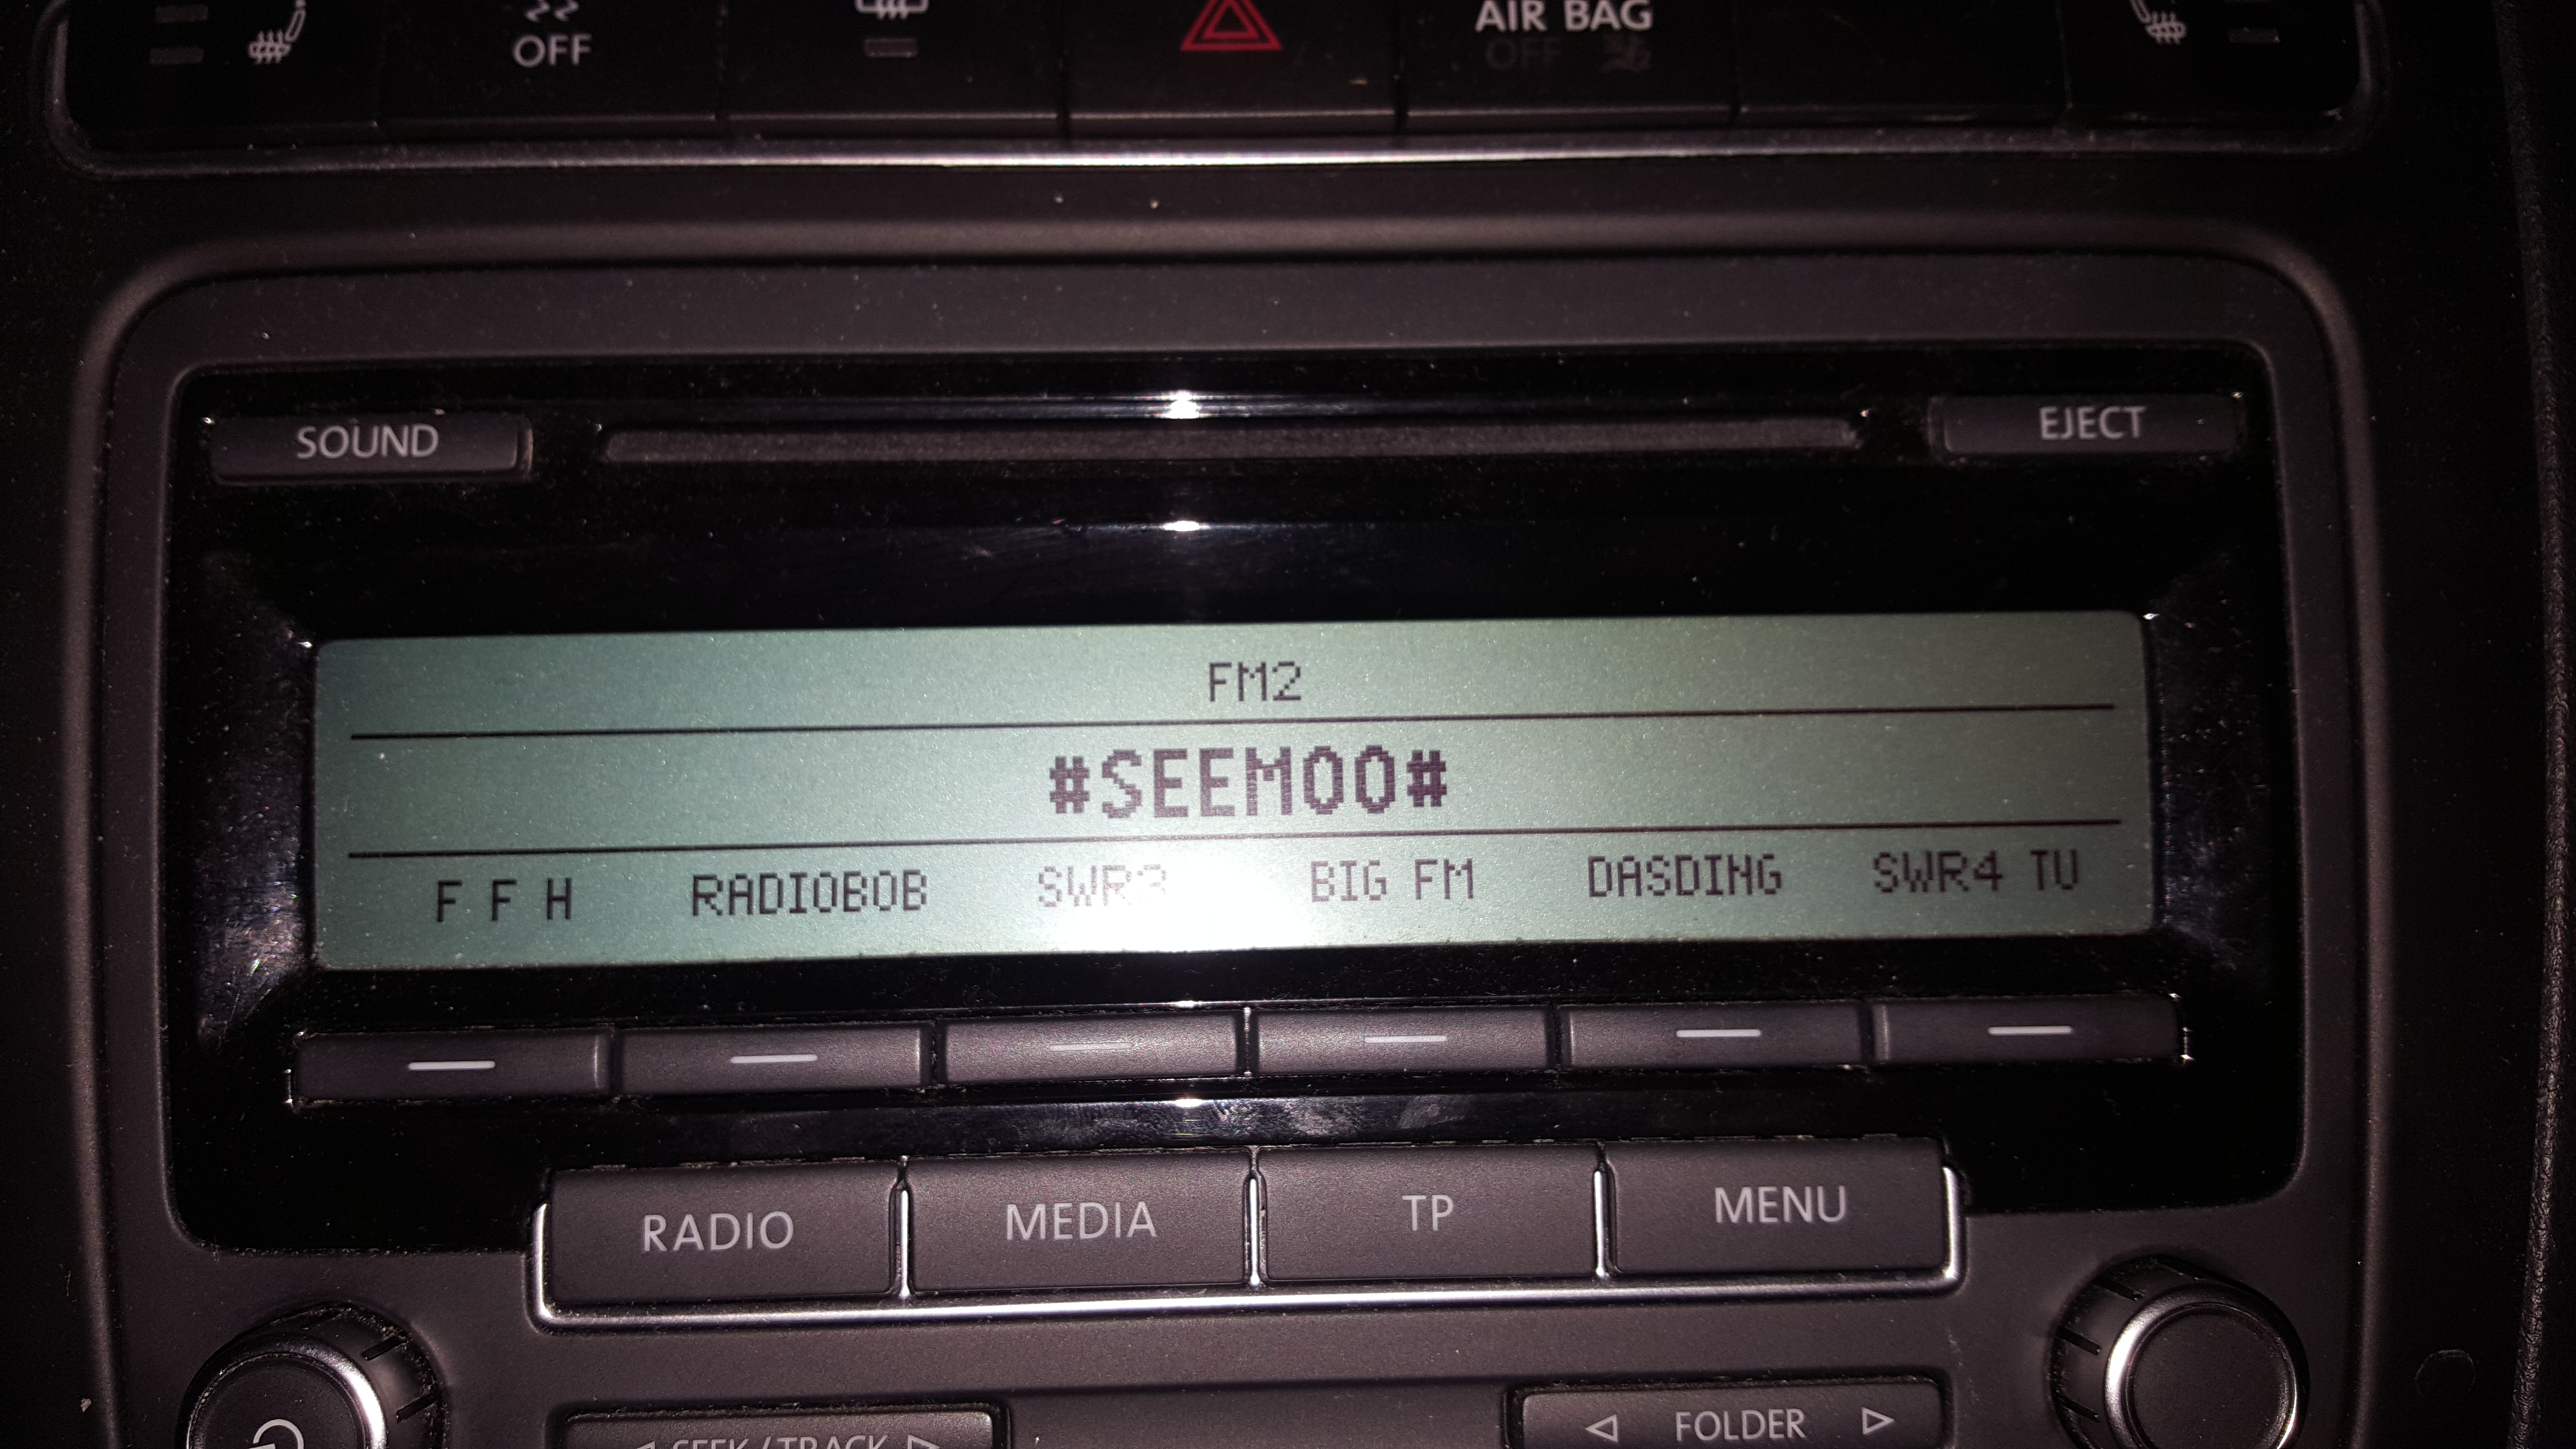
\includegraphics[width=1.0\linewidth]{gfx/feature2_pic.jpg}
	\caption{Decoded RDS signal on car radio}
	\label{fig:impl:picrds}
\end{figure}

\subsection{Optimization}
Since the modulation of the RDS signals requires quite some computation we decided to do the calculation until step 7 before the actual transmission is started. This precalculated RDS frame does not change over time, so we can just reuse it in every new SamplePacket that is requested. The actual getNextSamplePacket() then only retrieves the audio samples (from file or from microphone), adds them to the RDS frame and does the frequency modulation. This computation can be done in real time without any problems. 

Since our transmission chain and the HackRF work with 1 MHz sampling rate, we initially also used 1MHz to calculate the RDS signals. This however, proved to be extremely expensive. Especially the filtering of the signal does require a lot of time. This resulted in a precalculation time of up to 6 seconds even on our high end testing devices. Since the signal only contains frequencies up to around 60 kHz, we do not require such a high sampling rate. We improved the code (basically steps 4 to 7) to work with a variable sampling rate. After step 7 the signal is then upsampled to 1 MHz, such that the real time computation (step 8 and 9) stays unchanged.

To keep the upsampling step easy (both from implementation and computational view), we only used factors of 1 MHz. We tested 500 kHz, 250 kHz, 200 kHz and 125 kHz. However, for 125 kHz, the signal was no longer decodable by our testing radio. Therefore, we used 200 kHz as the lowest sampling rate. 


\begin{table}

	\caption{RDS Optimization: Using different sampling rates for the calculation of 4x4 RDS groups (around 1400ms)}
		\label{tab:rds_optimization}
	
	\begin{tabular}{c | p{4cm} | p{4cm} }
		sampling rate &  avg. execution time (Samsung Galaxy S6) & avg. execution time (Google Nexus 6p) \\ \hline
		1MHz	& 4840 ms & 5684 ms \\ \hline 
		500kHz	& 1340 ms & 1566 ms \\ \hline
		250kHz 	& 441 ms  & 480 ms\\ \hline
		200kHz 	& 339 ms  & 340 ms 
		
	\end{tabular}
\end{table}

We performed experiments on how the sampling rate affects the execution time. The results are shown in Table~\ref{tab:rds_optimization}. Since the experiments are performed on physical devices, the processor might also be busy with other computations. Therefore, we repeated the experiment five times for each sampling rate and device and used the mean value (the variance was small for all measurements).  We see that the sampling rate drastically affects the performance. We have been able to reduce the computation time from 4840 ms on the Galaxy S6 (or 5684 ms on the Nexus 6p) to 339 ms (340 ms). This is a performance gain of 1328\% (1572\%).  
With the optimized implementation we could in theory do the modulation in real time and ahead of the transmission start. However, since we also need to do other computation and we do not want to unnecessarily strain the smartphone, we did not change that part. 

\section{Feature 3: Walkie Talkie} 

AnSiAn in the version of December 2016 is capable of receiving and demodulating analogue signals, transmitting and receiving simple digital signals and now even implemented the first advanced digital protocol. However, it stills lacks the ability to transmit analogue signals. This is implemented as a part of feature 3. 
\begin{figure}
	\centering
	\includegraphics[width=1.0\linewidth]{gfx/feature3_concept.pdf}
	\caption{Design of the Walkie Talkie Feature (Simplified Tx and Rx chain)}
	\label{fig:impl:f3concept}
\end{figure}

Since AnSiAn with this feature is capable of providing all functionality of an amateur radio walkie talkie, we call this feature Walkie Talkie and extend AnSiAn with an additional view that provides modest access to this feature. Figure~\ref{fig:impl:f3concept} shows the components that are required for this feature. First, we need a new view called "WalkieTalkieView". This view basically allows the user to switch between reception and transmission mode. Then, either the reception chain or the transmission chain is active. The reception chain retrieves samples from the HackRF, demodulates them and plays the audio signal using the built in speakers. The reception chain is already fully implemented in the previous version of AnSiAn. So, only very minor changes are required here. 
The transmission chain records samples from the integrated microphone, modulates them and transmits them with the HackRF. Most required parts here have been implemented in Feature 1 (see Section~\ref{sec:impl:feature1}). However, we need to implement new modulations here. We want to implement FM, LSB and USB. FM will be integrated, because it was already used in feature 2 (Section~\ref{sec:impl:feature2}), and therefore, we expect the implementation to be straightforward. LSB and USB will be integrated because they are the most widely used modulation schemes in amateur radio. 

\subsection{User Interface}
\begin{figure}
	\includegraphics[width=1.0\linewidth]{gfx/screenshot_walkietalkie.png}
	\caption{AnSiAn WalkieTalkie Tab: FM (left) and USB (right)}
	\label{fig:impl:f3ui}
\end{figure}

Figure~\ref{fig:impl:f3ui} shows the new WalkieTalkie tab implemented as a part of this feature. On the left side you can see the UI when using FM and on the right side is the UI when using USB (or LSB). The only difference is that, when using USB or LSB, the user can specify the width of the filter applied to the signal (see Section~\ref{subsubsec:lsbusb}). To ease the selection of a legal amateur radio frequency, we provide a selection of popular frequency bands that can be used legally in Germany if the user possesses an amateur radio license \cite{afuv}: 
\begin{itemize}
	\item 80m Band (3.5MHz - 3.8MHz)
	\item 60m Band (5.3MHz - 5.4MHz)
	\item 40m Band (7.0MHz - 7.2MHz)
	\item 30m Band (10.1MHz - 10.2MHz)
	\item 20m Band (14.0MHz - 14.4MHz)
\end{itemize}

The choice of the frequency might depend on various factors, e.g. used antenna, hardware of communication partner, frequency occupancy and intended communication range. 
Additionally, we provide a "other" band, which enables the user to freely choose a frequency within the range supported by HackRF (1 MHz to 6 GHz). However, the user is responsible for using this feature legally. To fine tune the frequency the user can use a seek bar to select a frequency within the selected band. 

After selecting the frequency band, the user can select one of three modulation schemes, namely FM, LSB and USB. Usually LSB is used for frequencies below 10 MHz and USB is for frequencies above. However, we let the user decide which modulation scheme he wants to use.
The settings for Amplifier, Antenna Port Power and VGA Gain are parameters for the HackRF hardware, that can be used to optimize the transmission/reception quality. Since they are the same as in the TransmitView, we do not explain them in detail here and refer to \cite{Mantz2016}. 

The last parameter that can be set in the WalkieTalkieView is the squelch threshold setting. It is used to suppress noise when there is no signal. 
\begin{figure}
	\centering
	\includegraphics[width=0.8\linewidth]{gfx/walkietalkieview_fsm.pdf}
	\caption{State Machine of WalkieTalkie View}
	\label{fig:impl:f3fsa}
\end{figure}

At the bottom of the screen, there are two buttons to start/stop reception and transmission. Since we cannot receive and transmit at the same time. We need to switch between these modes. We assume a classical walkie talkie use case, where we receive for the majority of the time and switch to transmission mode for short periods in between. Therefore, we implemented the state machine shown in Figure~\ref{fig:impl:f3fsa}. 

At first, the radio is turned off and the user can enter the parameters. Then, the transitions 1 to 4 are straightforward:  The user can either enable RX or TX. Accordingly, the reception or transmission is started. By pressing the same button again, the radio is turned of again. The other transitions are similar to the behavior we would expect from a walkie talkie: 
\begin{itemize}
	\item \textbf{Transition 5} - The HackRF is in transmission mode and the user pressed the RX button: No action is taken, but a RX flag is set, such that once the transmission is stopped, we change into reception mode and not off. 
	\item \textbf{Transition 6} - The HackRF is in transmission mode, the RX flag is set and the user presses the RX button: No action is taken, but the RX flag is unset, such that the reception is not resumed once the transmission is stopped. 
	\item \textbf{Transition 7} - The HackRF is in reception mode and the user presses TX: The reception is paused and the transmission is started. 
	\item \textbf{Transition 8} - The HackRF is in transmission mode, the RX flag is set and the user presses TX: The transmission is stopped and the reception is resumed. 
\end{itemize}

A classical state transition flow would be 3, 7, 8, 4. 
\subsection{Implementation}

This section describes the required changes in the reception and transmission chain of AnSiAn. 
Since the reception of FM, USB and LSB was already implemented in the last version, the only task here was to correctly call the API of the reception chain. For setting the required parameters (e.g. frequency) AnSiAn uses Android Preferences, which handle the serialization and deserialization of the settings to/from a file to persist the the settings beyond the runtime of Android applications. For more details we refer to the Android documentation \cite{androidpref} and the documentation of the first AnSiAn version \cite{Kreis2015}.

The start of the reception is then initiated by posting a RequestStateEvent to the EventBus (which is a publish/subscribe library by greenrobot). The communication within AnSiAn is mainly based on such events. For greater details on the large variety of available events in AnSiAn, we again refer to \cite{Kreis2015}. The only change required in the reception chain was to extend the preferences, such that a custom filter bandwidth can be specified for the LSB and USB demodulation. 

The most changes for this feature were required in the transmission chain. Firstly, we needed to generalize the recording of audio from the microphone from the RDS feature. Additionally, we implemented the three Modulation schemes FM, LSB and USB. FM was already used for RDS, so we just needed to generalize the implementation and exclude the RDS signals. LSB and USB are newly added. The following sections describe some key aspects in greater detail. 

\subsubsection{AudioSource}

For all three modulations it is required to retrieve PCM samples from the microphone. We implemented this functionality in the self-contained AudioSource class, such that it can also be used in other scenarios. Basically the class provides three methods: One for starting the collection of audio samples (startRecording()), one to retrieve the audio samples (getNextSamples()) and one to stop the recording and release the resources (stopRecording()). 

\begin{lstlisting}[label=lst:javaaudiorecord, caption=Retrieving PCM samples from microphone, language=java,]
public class AudioSource {
//...
 private int AUDIO_SOURCE = MediaRecorder.AudioSource.MIC;
 private int AUDIO_SAMPLERATE = 44100;
 private int AUDIO_CHANNELS = AudioFormat.CHANNEL_IN_MONO;
 private int AUDIO_ENCODING = AudioFormat.ENCODING_PCM_FLOAT;

 public boolean startRecording(){
    this.recorder = new AudioRecord(AUDIO_SOURCE,
	AUDIO_SAMPLERATE, AUDIO_CHANNELS,
	AUDIO_ENCODING, this.bufferSize*4);
    this.recorder.startRecording();
    // ... error handling ... 
 }

 public float[] getNextSamples(){
    if(this.recorder == null) return null;
    float[] buffer = new float[this.bufferSize];
    this.recorder.read(buffer, 0, buffer.length, AudioRecord.READ_BLOCKING);
    return buffer;
 }
 //...
}
\end{lstlisting}
Luckily, Android does provide a API to retrieve float PCM samples through the AudioRecord class \cite{androidaudio}. Listing~\ref{lst:javaaudiorecord} shows the implementation of startRecording() and getNextSamples(). For the purposes of presentation, some implementation details for error handling have been removed.  An instance of AudioRecord can be created using the following parameters: 
\begin{itemize}
	\item \textbf{audioSource}: MediaRecorder.AudioSource.MIC is the most reasonable for us. Other options are uplink and/or downlink of a current call. 
	\item \textbf{sampleRateInHz}: 44100 Hz is guaranteed to work on all devices. Some devices might provide other sample rates as well.
	\item \textbf{channelConfig}: Mono is guaranteed to work on all devices. Stereo might not be supported.
	\item \textbf{audioFormat}: We use floats, since our entire modulation works with floats. Other options would be 8-bit (i.e. bytes) or 16-bit (i.e. shorts). 
	\item \textbf{bufferSizeInBytes}: size of internal buffer. We use a default value of 32 KiB. 
\end{itemize}

If the initialization (line 9) finishes successfully, the recording can be started using startRecording() (line 12). From now on Android fills up the buffer and we need to make sure that we retrieve the samples in time. Otherwise the buffer becomes full and Android throws away audio samples. 

The retrieval of audio samples is implemented in the getNextSamples() method. It allocates a new float buffer and calls the read method on the AudioRecord. Since Android API Level 23 (6.0 / Marshmallow) this can be called with a AudioRecord.READ\_BLOCKING argument, such that the call blocks until enough audio samples are available to fill the buffer. This simplifies our implementation, since we want the Modulator to block until enough samples are available. If we wanted to support lower API levels, we would need to implement this blocking behavior ourselves.

Additionally, to this getNextSamples() method, we provide two other methods to retrieve the samples: getNextSamplesUpsampled() (returns the samples upsampled to a higher sampling rate, which is specified in the constructor) and  getNextSamplePacket() (returns a SamplePacket instead of a float array).

\subsubsection{FM}

The central method that needs to be implemented for each modulation is the getNextSamplePacket() method, which is repeatedly called by the modulator until null is returned or the transmission is stopped. Using the fmmod from Section~\ref{sec:impl:feature2} and the AudioSource class, a frequency modulation implementation is straightforward. 

\begin{lstlisting}[label=lst:javafm, caption=Modulating microphone samples using frequency modulation, language=java,]
@Override
public SamplePacket getNextSamplePacket() {
	if(this.audioSource == null) return null;
	float[] upsampled = this.audioSource.getNextSamplesUpsampled();
	if(upsampled == null) return null;
	SamplePacket resultPacket = FM.fmmod(upsampled, sampleRate, 75000);
	return resultPacket;
}
\end{lstlisting}

Listing~\ref{lst:javafm} shows the basic steps. Firstly, the audio samples are retrieved from the AudioSource (l. 4). This might block until enough samples are available. Since this audio is sampled with 44100 Hz, we need to upsample the signal to 1MHz. This is already integrated in the AudioSource class with the getNextSamplesUpsampled(). If an error occurs during the retrieval of the samples, null is returned and we also return null to the Modulator (l. 5). This will cause the transmission to stop. Otherwise we pass the upsampled signal to fmmod, which implements the frequency modulation (l. 6). 

\subsubsection{LSB/USB}
\label{subsubsec:lsbusb}
\begin{figure}
	\centering
	\includegraphics[width=1.3\linewidth]{gfx/ssb_plots.png}
	\caption{Time Domain and Frequency Domain of AM, LSB and USB Signals}
	\label{fig:impl:f3ssb}
\end{figure}


In amateur radio the most widely used modulation schemes is single side band modulation, which is a advancement of amplitude modulation. Figure~\ref{fig:impl:f3ssb} illustrates why this is done. It contains the time and frequency domains of a modulated audio signal (to be more exact: the Star Wars Imperial March). Subplot 1 contains the time domain of the source signal. Subplot 2 shows the frequency domain of this signal. Since we are working with complex signals, we have positive and negative frequencies which are mirrored at 0 Hz. This is no problem in the baseband (red), but when upmixing this signal to the carrier frequency (green), we see that both sidebands are upmixed. This has two disadvantages: Firstly, it is a waste of transmission power, since the second sideband does not contain additional information. Secondly, our signal occupies more bandwidth, which is a very rare resource. 
This problem is solved by SSB. We either use the upper sideband (positive frequencies) or the lower sideband (negative frequencies). The ideal frequency domains are shown in Subplot 2 and 3. 

There are multiple ways to implement SSB modulation. The plots in Figure~\ref{fig:impl:f3ssb} are generated in Matlab using the Hilbert transformation to create a complex signal and then multiplying the imaginary part by either i (USB) or -i (LSB). However, this requires both the implementation of the Hilbert transformation and the complex multiplication, both is currently not available in AnSiAn. 

\begin{lstlisting}[label=lst:javassb, caption=Modulating microphone samples using SSB, language=java,]
@Override
public SamplePacket getNextSamplePacket() {
  // get audio samples
  SamplePacket packet = audioSource.getNextSamplePacket();
	
  if(packet == null) return null;
	
  // filter out the upper or lower side band
  ComplexFirFilter filter = ComplexFirFilter.createBandPass(1,1, audioSource.getAudioSamplerate(),
	isUpperSideband ? 0 : -this.filterBandWidth,
	isUpperSideband ? this.filterBandWidth: 0,
	audioSource.getAudioSamplerate()*0.01f, 40);
	
  SamplePacket output = new SamplePacket(packet.size());
  filter.filter(packet,output, 0, packet.size());
	
  // upsample from audio frequency (usually 44.1kHz) to our transmission frequency (1MHz)
  SamplePacket upsampled = output.upsample((int) Math.ceil((float) this.sampleRate / audioSource.getAudioSamplerate()));
  return upsampled;
}
\end{lstlisting}


Therefore, we decided to use a filter to get rid of the other sideband. Listing~\ref{lst:javassb} shows the implementation of the SSB in AnSiAn. Firstly, we retrieve the next audio samples from the AudioSource (l. 4). Then, we filter out the band we want using a ComplexFirFilter (the arguments are similar to the FirFilter used in Section~\ref{sec:impl:feature2}). When using USB, the pass band of the filter is from 0 Hz to the user defined filter bandwidth, e.g. 3000Hz. When using LSB this would be -3000Hz to 0 Hz. The resulting packet is then upsampled to 1MHz and returned to the modulator. 

Note: The AudioSource does return a real signal, not a complex signal, i.e. all imaginary parts are zero. However, the filter does correct this, such that the output signal does contain both a real and an imaginary part.

\section{Feature 4: Slow-scan Television (SSTV)}

\begin{figure}
	\centering
	\includegraphics[width=\linewidth]{gfx/sstv_intro.png}
	\caption{Modulation of \ac{SSTV}  signals - frequency domain of sync and line sequences \cite[p. 239]{pritchard2016newnes}}
	\label{fig:impl:sstv:intro}
\end{figure}

\subsection{User Interface}

\begin{figure}
	\centering
	\includegraphics[width=0.4\linewidth]{gfx/screenshot_gui_sstv.png}
	\caption{AnSiAn \ac{SSTV} View - Tx only}
	\label{fig:impl:sstv:gui}
\end{figure}

\subsection{Implementation}
\subsubsection{Modulation}
\begin{figure}
	\centering
	\includegraphics[width=1.0\linewidth]{gfx/screenshot_rxsstv.png}
	\caption{Validation of our modulation using a free SSTV decoder \cite{rxsstv}}
	\label{fig:impl:sstv:rxsstv}
\end{figure}

\subsubsection{Demodulation}

\begin{figure}
	\centering
	\includegraphics[width=1.0\linewidth]{gfx/sstv_nice.jpg}
	\caption{Frequency domain of the transmitted signal - showing the start of a frame (frame sync, line, line sync, line, line sync, line)}
	\label{fig:impl:sstv:spectro_tx}
\end{figure}

\begin{figure}
	\centering
	\includegraphics[width=1.0\linewidth]{gfx/sstv_rxside.jpg}
	\caption{Frequency domain of the received signal - showing the start of a frame (frame sync, line, line sync, line, line sync, line)}
	\label{fig:impl:sstv:spectro_rx}
\end{figure}

